%% TODO: Add line numbers to motivation example snippets, and update section.

\section{Motivation}
\label{intro:sec}

One of the drawbacks in \tdcleaner is that it's designed to learn
the correlations between inputs of different modalities, i.e., source 
code, and natural language. In this section, we illustrate several 
examples that align with the hypotheses described earlier, where
the  code-change resolves the TODO comment, for which, however, 
\tdcleaner still predicts that it is not obsolete, i.e., has not been 
performed by the developer. Figure~\ref{fig:mex_1} illustrates an 
example in which the TODO comment recommends the developers to ensure that 
the item that is to be appended to the {\em''Backpack''} menu is a valid 
game item. This is adopted, and added through the {\em if-statement} 
(on Line \_\_) in the code-change indicating a concordance between 
the code-change  and the TODO comment. However, the commit 
message in this illustration is very vague, indicating some fix to 
the {\em''Backpack''} menu, which is not in accordance with the TODO 
comment. Such  a non-accordance misleads \tdcleaner towards 
classifying the example as non-obsolete. 

\begin{figure}[t]
	\centering
	\begin{subfigure}{.45\textwidth}
		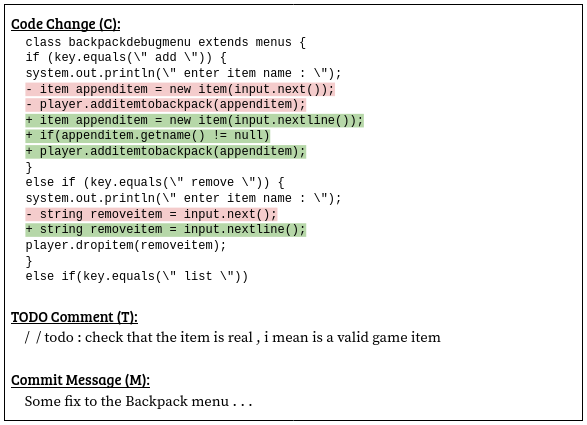
\includegraphics[width=\textwidth]{images/mex_1.png}
		\caption{$T \leftrightarrow C$, $T \nleftrightarrow M$}
		\label{fig:mex_1}
	\end{subfigure}
%%%%%%%%%%%%%%
	\begin{subfigure}{.45\textwidth}
		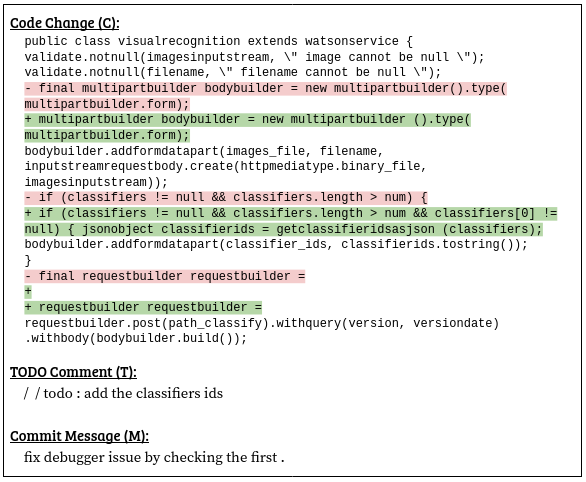
\includegraphics[width=\textwidth]{images/mex_2.png}
		\caption{$T \leftrightarrow C$, $M \geq T$}
		\label{fig:mex_2}
	\end{subfigure}
%%%%%%%%%%%%%%
	\begin{subfigure}{.45\textwidth}
		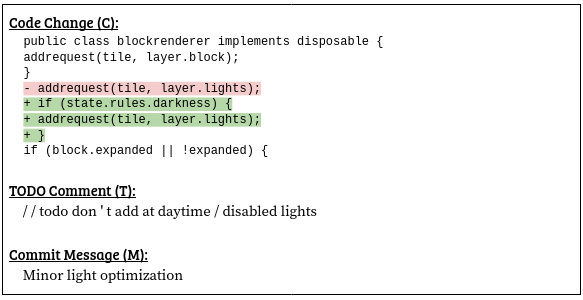
\includegraphics[width=\textwidth]{images/mex_3.png}
		\caption{$T \leftrightarrow C$, $M \geq C$}
		\label{fig:mex_3}
	\end{subfigure}
\caption{Motivating Examples.}
\end{figure}

Figure~\ref{fig:mex_2} illustrates an example in which the TODO comment is
in concordance with the code change, but the commit contains other 
changes as well. The TODO comment recommends the developers 
to add classifier IDs, which is clearly addressed in the statement 
block within the {\em if-statement} on Line \_\_. However, the commit, on 
the whole fixes a debugger issue by adding an additional condition 
to the {\em if-statement}, i.e., by also ensuring that the first element in 
the classifier is not null. This change, overall, also aligns with the 
commit message logged by the developer.

In the example illustrated in Figure~\ref{fig:mex_3}, a developer added a 
TODO comment, to recommend the team to not add requests to a 
block at daytime. This was addressed by introducing a check for 
darkness before adding requests, through the {\em if-statement} on Line
\_\_. However, the corresponding commit message that was logged
for this code modification was very general, indicating a minor
light optimization, which doesn't entirely explain/summarize the 
changes in code. Thus, the contextualized vector learnt for the 
commit message might have acted as noise, influencing \tdcleaner to
predict that the TODO comment in this instance was not addressed
by the developers. 

Such inconsistencies motivated us to explore approaches to 
untangle the $<T, C, M>$ triples, and build individual tasks utilizing 
parts of the triples, each modeled towards detecting obsolete TODO 
comments. This idea forms the crux of \tool, which we'll 
go over in more detail in the following sections.
